\section{Results}

Here, one can display figures, such as in \Cref{fig:example}.

Each assessment was done with the following target coordinates.

\begin{table}[]
    \begin{tabular}{|l|l|l|l|l|l|l|l|l|l|l|}
    \hline
    \textbf{Target} & \textbf{1} & \textbf{2} & \textbf{3} & \textbf{4} & \textbf{5} & \textbf{6} & \textbf{7} & \textbf{8} & \textbf{9} & \textbf{10} \\ \hline
    \textbf{x}      & 0.35       & -0.35      & 0.5        & -0.35      & 0.35       & -0.15      & -0.35      & 0.35       & -0.5       & 0.35        \\ \hline
    \textbf{y}      & 0.3        & 0.4        & -0.4       & 0          & 0.4        & -0.1       & -0.3       & -0.4       & 0.4        & 0           \\ \hline
    \end{tabular}
\end{table}

Each simulation was also run for 3000 simulation steps.

In this simulation, the heuristic algorithm hit 5 targets and achieved a value for the sum of rewards as 4894.42, against our chosen reward function.
The following graph shows an example of the Soft state Monti-Carlo state machine algorithm’s results, under the same conditions.

We modelled the cumulative reward function for any given epoch using the least-sqares optimized log function.

1475.01044  *ln(0.00310817391*CumReward)+ 1642.65857 




\begin{figure}
    \centering
    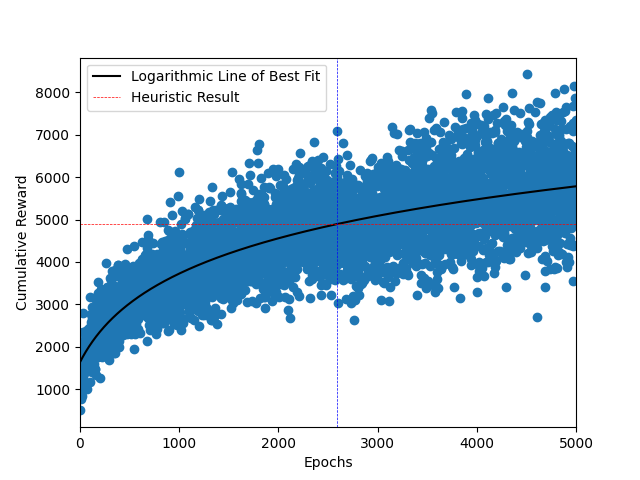
\includegraphics[width=\singlefigure]{figures/figure_2.png}
    \caption{\label{fig:example} Shows an example of a figure.}
\end{figure}

\begin{figure}
    \centering
    \includegraphics[width=\singlefigure]{figures/figure_3.png}
    \caption{\label{fig:example} Shows an example of a figure.}
\end{figure}